\section{设计}
\label{sec:design}

本节介绍 \sys 的系统设计。我们首先给出 \sys 使用的数据结构，并说明块稀疏行（BSR）如何成为注意力内核中 KV cache 存储的通用抽象。随后介绍 \sys 编译器：它支持多类注意力变体，并配合一个感知动态输入的运行时调度器，实现注意力内核的负载均衡调度。最后，我们描述面向用户的 API，以便将 \sys 集成到现有 LLM 服务系统中。

\subsection{KV-Cache 存储}

\subsubsection{将块稀疏矩阵作为统一格式}

近期 KV-Cache 存储方案（如 PageAttention~\cite{kwon2023vllm}、RadixAttention~\cite{zheng2023sglang}）通常采用非连续内存布局，其最小粒度为一个 $(H, D)$ 的张量块（或 token），其中 $H$ 是头数，$D$ 是隐藏维度。这些结构旨在最小化内存碎片，同时提高复用率与缓存命中率。我们表明，这些异构数据结构都可在块稀疏格式下统一表示，如图~\ref{fig:focus-sparse-layout} 所示。

\begin{figure}[ht]
    \centering
    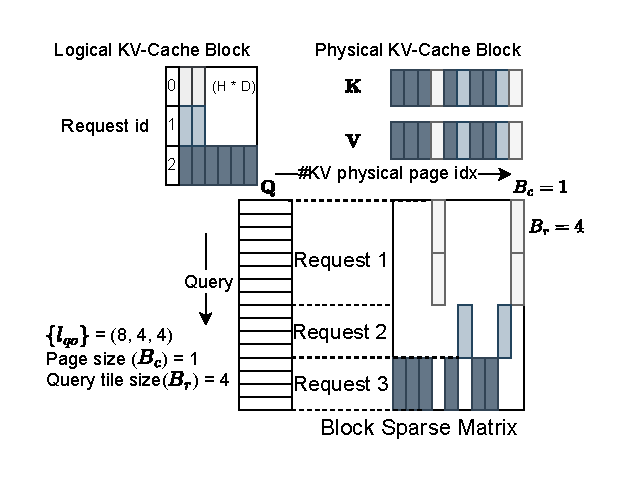
\includegraphics[width=0.45\textwidth]{figures/flashinfer-sparsetir-format.pdf}
    \caption{将页表表示为 BSR $(B_r=4,B_c=1)$ 格式。块稀疏矩阵的列块数对应页表已分配块的总数；非零块表示 query 会访问到的 KV-Cache 页面。}
    \label{fig:focus-sparse-layout}
\end{figure}

将页表与稀疏矩阵在概念上等价化的思路在 SPGrid~\cite{setaluri2014spgrid} 中已有探索，其借助 TLB 硬件高效索引稀疏结构。除页表与基数树外，稀疏矩阵也能表达多种注意力机制，例如推测解码中的树注意力~\cite{cai2024medusa,miao2023specinfer,chen2024sequoia}，以及施加在 KV-Cache 上的重要性掩码~\cite{tang2024quest}。

在 \sys 中，我们采用统一数据表示策略。query 与 output 使用无 padding 的 ragged tensor（又称 jagged array）~\cite{ragged-tensor} 存储，便于将不同请求的 query/output 紧凑打包到同一张量。初始时，key/value 也使用与 query 相同索引指针的 ragged tensor（因为它们来自同一输入经 $W_q,W_k,W_v$ 投影）。随后，这些 key/value 会写入 KV-Cache 并更新索引。KV-Cache 采用 BSR 格式，块大小由应用决定：$B_r$ 对应 query tile 大小（后文介绍），$B_c$ 由 KV-Cache 管理算法给出。\sys 内核支持任意 $(B_r, B_c)$。

\begin{figure}[ht]
    \centering
    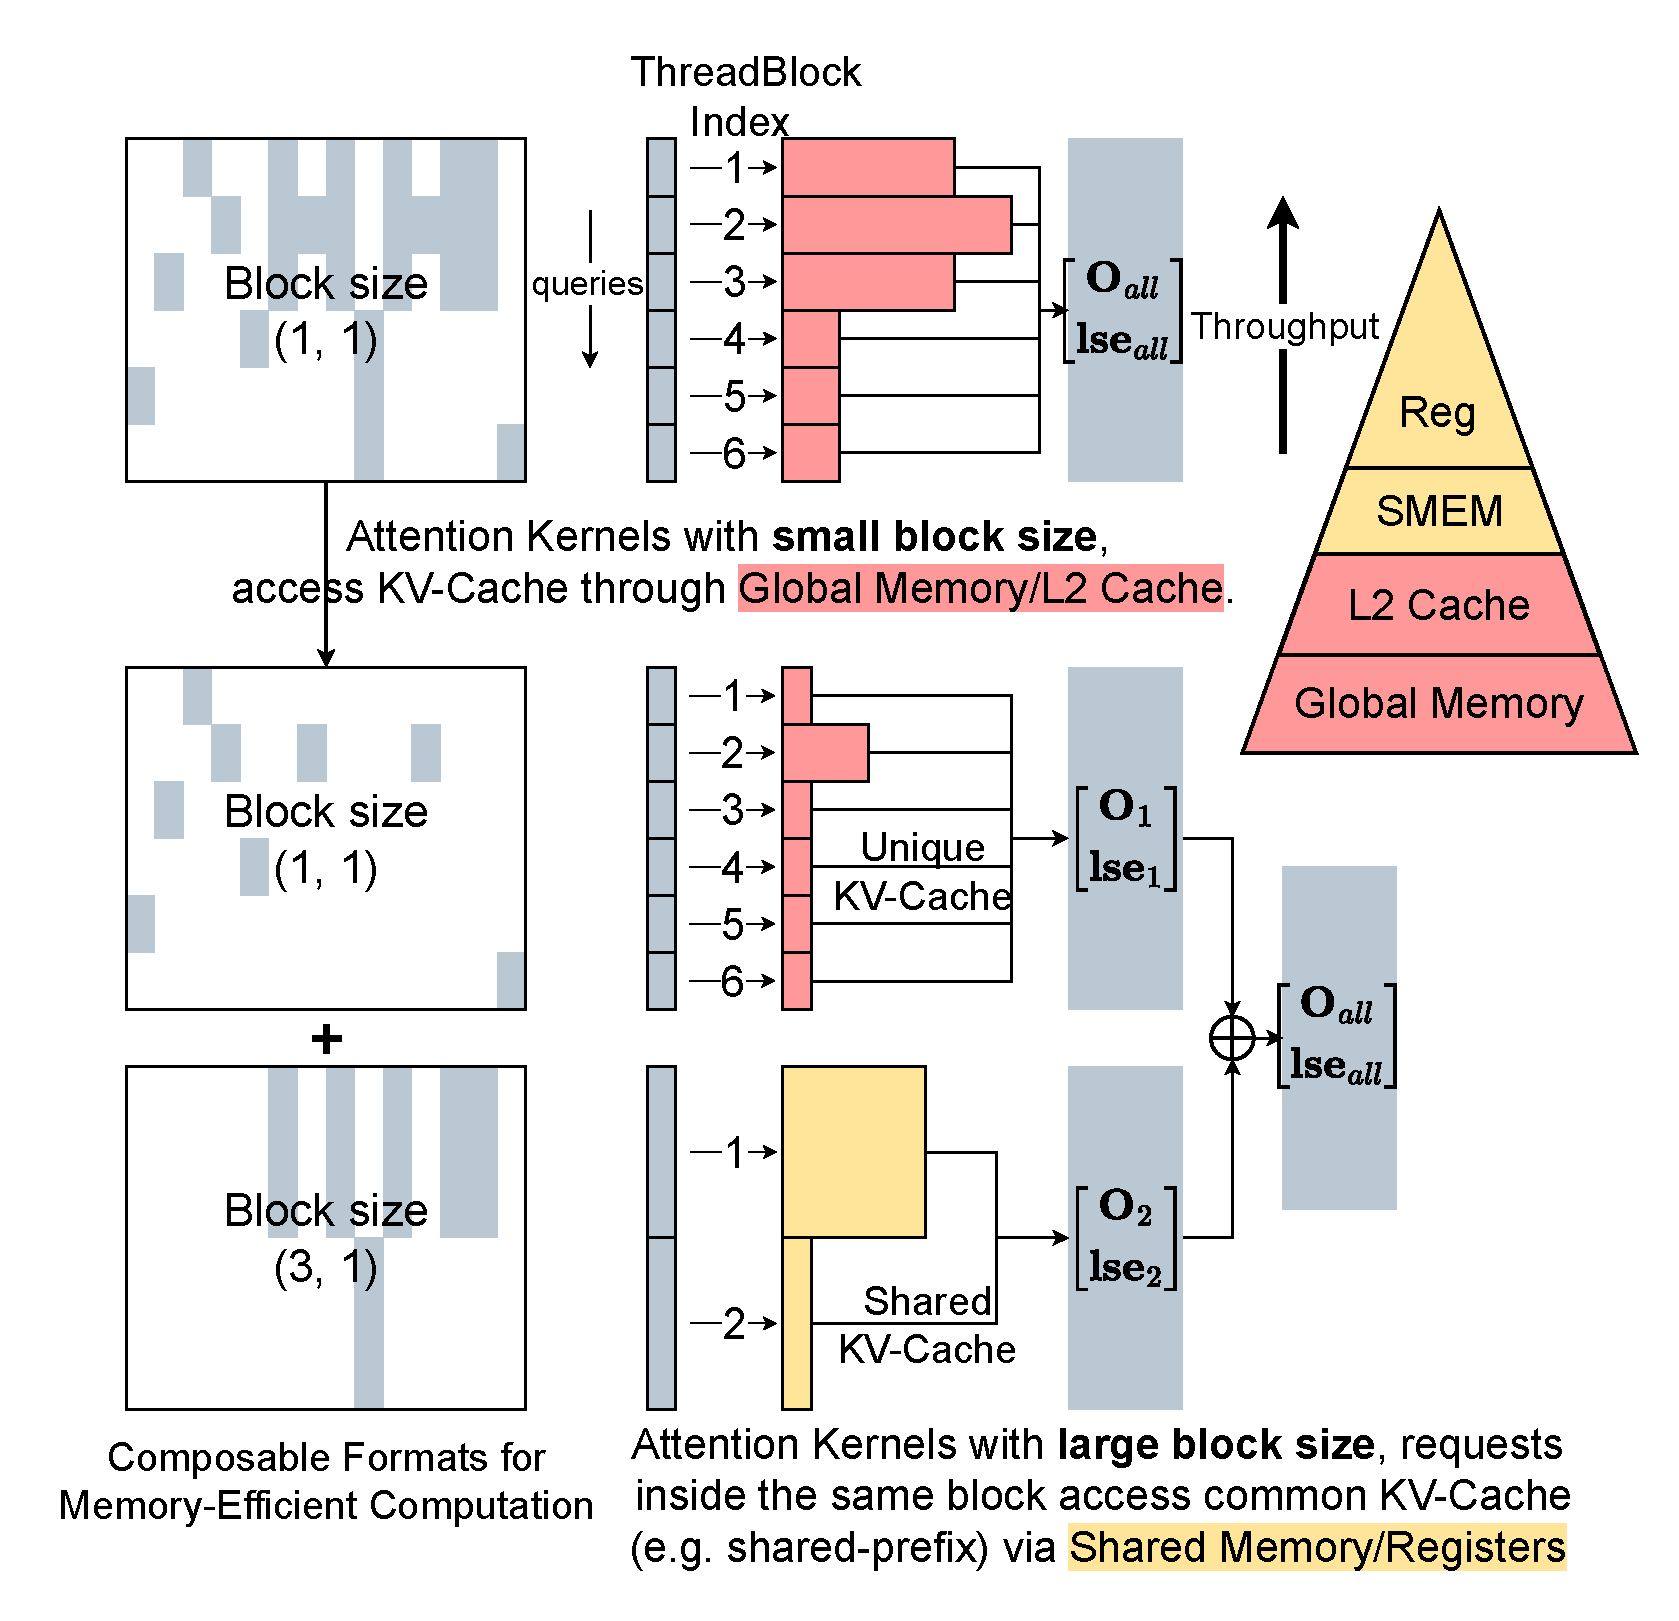
\includegraphics[width=0.45\textwidth]{figures/flashinfer-composable-formats.pdf}
    \caption{用于共享前缀分解的可组合格式。前 6 行 query 共享前缀，后 6 行 query 也共享前缀。我们用块大小 $(3,1)$ 的块稀疏矩阵存储共享前缀对应的 KV cache，用块大小 $(1,1)$ 的块稀疏矩阵存储其余非共享 KV cache。对于 $(3,1)$，3 个 query 可在高带宽共享内存中复用同一 KV cache；对于 $(1,1)$，每个 query 只能在各自 threadblock 内访问 KV cache，路径仅能走低带宽全局内存或 L2。}
    \label{fig:flashinfer-composable-formats}
\end{figure}
\subsubsection{用于内存效率的可组合格式}
\label{sec:composable-formats}

受 SparseTIR~\cite{ye2023sparsetir} 启发，我们通过可组合格式提升注意力计算效率。其核心是使用多个块稀疏格式共同存储一个稀疏矩阵，而非单一格式，从而在灵活性与内存效率上更优。单一块稀疏格式受固定块大小约束，其内存效率受块行数 $B_r$ 限制：较大 $B_r$ 可提升同块请求的共享内存与寄存器复用，但也会增大碎片；不同块之间又无法共享彼此的片上数据。

我们的可组合格式允许基于先验知识对 KV cache 稀疏矩阵进行分解。例如，若部分请求共享前缀，其对应行列会形成稠密子矩阵，此时可用更大 $B_r$ 的块稀疏矩阵高效表示。图~\ref{fig:flashinfer-composable-formats} 展示了这一思路。该方法无需移动 KV cache 数据，只需计算稀疏子矩阵的索引与索引指针数组。对较大块大小执行注意力计算时，可通过高速共享内存与寄存器复用共享 KV cache，显著提升内存效率。

\subsection{计算抽象}
\label{sec:compute-abs}

我们基于 CUDA/CUTLASS~\cite{cutlass} 开发了 FlashAttention 模板，面向稠密与块稀疏矩阵，并兼容 Turing 到 Hopper（sm75 到 sm90a）的 NVIDIA GPU。对于 Ada（sm89）及以下架构，我们采用 FlashAttention2（简称 FA2）算法~\cite{dao2023flashattention2}；对 Hopper，采用 FlashAttention3（简称 FA3）算法~\cite{jay2024flashattention3}。关键改进包括：更高效的稀疏 tile 共享内存加载、更丰富的 tile 大小配置、针对 GQA 的优化内存访问模式，以及可定制注意力变体支持。

\subsubsection{从全局内存到共享内存的数据搬运}
\label{sec:sparse-loading}

\sys 的注意力模板支持任意块大小，因此需要专门的数据加载机制，因为块形状可能与 Tensor Core 形状不对齐。正如第 \ref{sec:block-sparse} 节所述，我们通过将分散的全局内存 tile 搬运到连续共享内存，再执行稠密 Tensor Core 计算来解决该问题。一次 MMA 指令所需输入可能来自块稀疏矩阵中的不同块。图 \ref{fig:sparse-loading} 展示了 \sys 如何将稀疏/稠密 KV-Cache 的 tile 载入共享内存：稀疏 KV-Cache 地址通过 BSR 的 \texttt{indices} 数组计算，稠密地址通过行索引仿射变换计算。

KV-Cache 的最后一维保持连续（head dimension $d$，通常 128 或 256），从而维持与 GPU cache line 匹配的合并访存。我们采用 128B 宽度的异步拷贝指令 \texttt{LDGSTS} 以最大化内存带宽利用。尽管 Hopper 的 TMA（Tensor Memory Accelerator）可进一步加速数据搬运，但其不支持非仿射访问模式，因此仅在连续 KV-Cache 的 Hopper 场景使用 TMA；其他不适配场景回退至 Ampere 风格异步拷贝。

\begin{figure}[ht]
    \centering
    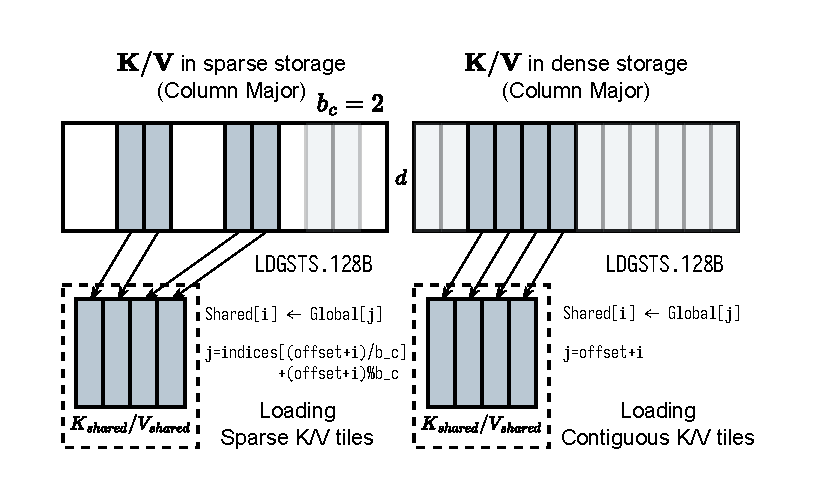
\includegraphics[width=0.45\textwidth]{figures/flashinfer-sparse-loading.pdf} 
    \caption{\sys 中稀疏/稠密 KV-Cache 从全局内存到共享内存的数据搬运。左：稀疏 KV-Cache，$b_c=2$；右：稠密 KV-Cache。head dimension 为 $d$。}
    \label{fig:sparse-loading}
\end{figure}

搬运到共享内存后，稀疏与稠密 FlashAttention 实现将汇合：仅数据加载模块不同，核心计算内核可统一复用。

\subsubsection{多 tile 大小微内核}
\label{sec:tile-size-selection}

为适配 LLM 应用中不断变化的操作强度，\sys 在多种 tile 大小上实现了 FA2。传统 FA2 常使用少量固定 tile（如 $(128,64)$），在 A100 prefill 上效果较好，但对短 query 的解码场景效率不足。某一架构的最优 tile 在另一架构不一定合适；例如 Ada（sm89）共享内存较小，大 tile 会影响 SM 占用。

\sys 提供 ${\{1, 16, 32, 64, 128\} \times \{32, 64, 128\}}$ 的 FA2 内核，并基于硬件资源与工作负载强度使用启发式选择：

\begin{enumerate}[itemsep=2pt,topsep=0pt,parsep=0pt]
\item 计算 batch 平均 query 长度（对 GQA，会将 query 长度与 head group 维融合，见附录 \ref{sec:head-group-fusion}），并选择不小于该长度的最小 query tile。
\item 将寄存器与共享内存约束表示为 K/V tile 大小的函数，在约束下最大化 SM 资源占用。
\end{enumerate}

\begin{figure*}[!ht]
    \centering
    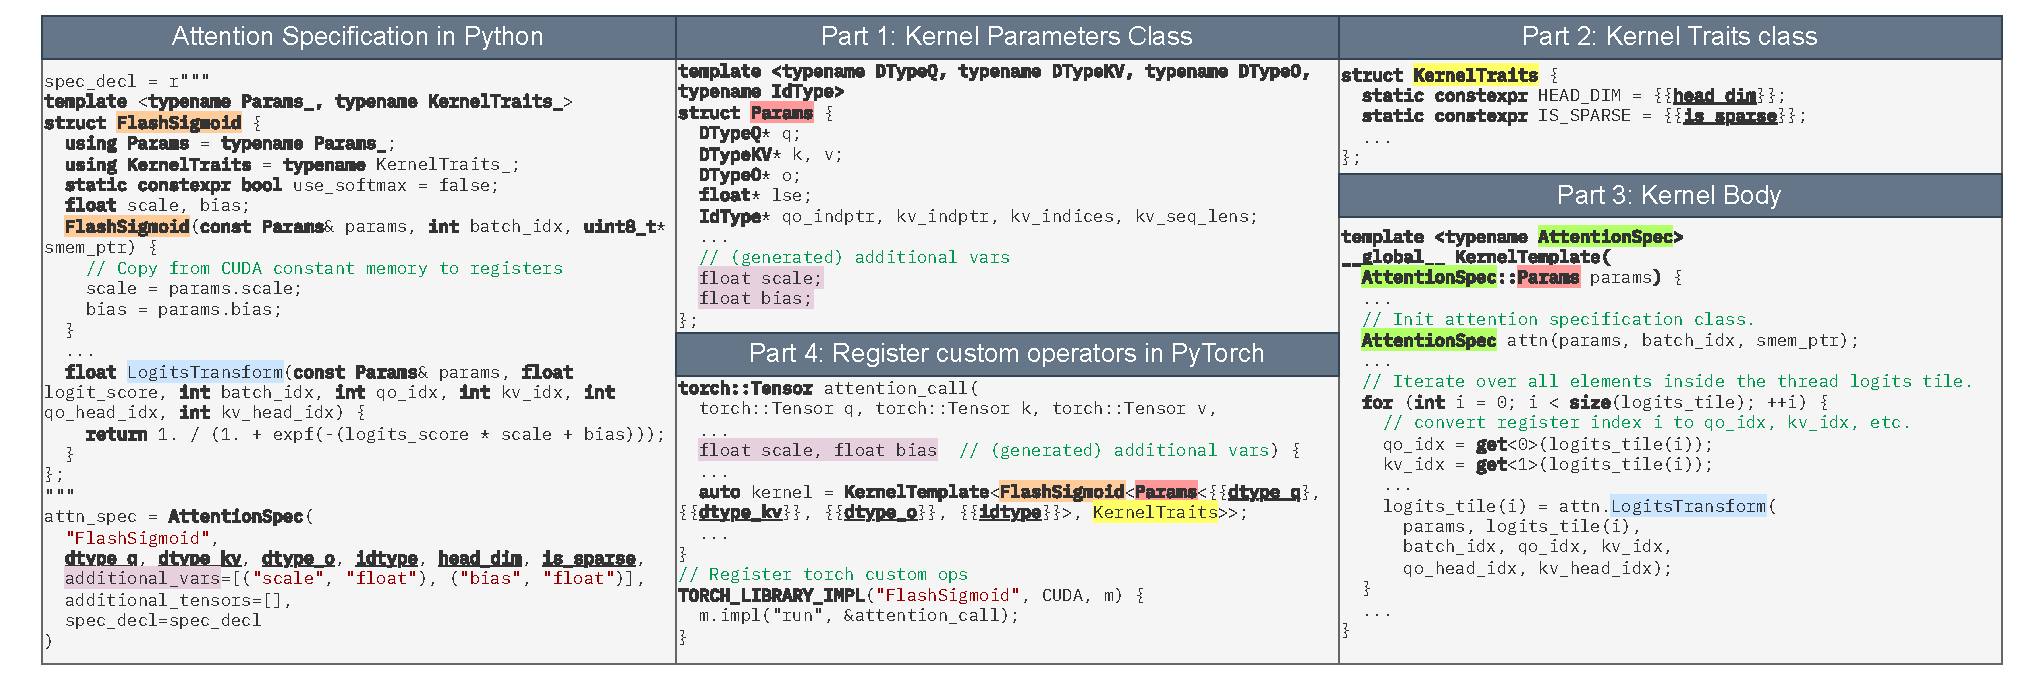
\includegraphics[width=1\textwidth]{figures/flashinfer-jit.pdf}
    \caption{\sys 的注意力变体 JIT 编译器：变体函子、附加变量/张量与数据类型由 CUDA 代码字符串定义，再用于填充内核模板；图中对应代码采用共享高亮。}
    \label{fig:flashinfer-attention-variants}
\end{figure*}
\subsubsection{面向注意力变体的 JIT 编译器}


当 query tile 为 1 时，我们使用 CUDA Core 模板（因为 Tensor Core 指令 $m$ 维最小为 16）；其余 query tile 大小使用 Tensor Core。对于 FA3，我们提供行 tile 为 64 倍数的配置以匹配 Hopper 的 WGMMA 要求。tile 大小在编译期结合任务类型（解码、prefill 等）和硬件能力确定。块稀疏矩阵的块行大小 $B_r$ 与 query tile 大小 $T_q$ 对齐。

近年的 LLM 广泛使用标准注意力的变体。若在 CUDA 库中逐一内建支持并针对每个变体专门优化内核，维护不可持续，而变体数量仍在快速增加。另一方面，大多数变体与标准注意力结构相近，因此可复用 FlashAttention 内核骨架，仅做小范围修改。受 FlexAttention~\cite{he2024flexattention} 启发，我们设计了可定制 CUDA 模板与 JIT 编译器：输入注意力变体规格后，自动生成优化内核代码。变体规格包含以下函子：

\begin{itemize}[itemsep=2pt,topsep=0pt,parsep=0pt]
    \item \texttt{QueryTransform, KeyTransform, ValueTransform}：注意力计算前施加在 query/key/value 上的变换。
    \item \texttt{OutputTransform}：返回前施加在注意力输出上的变换。
    \item \texttt{LogitsTransform, LogitsMask}：softmax 前施加在 logits 上的变换与掩码。
\end{itemize}

每个函子都有固定签名：输入为内核参数、输入张量及当前 query/key/head 索引，输出为变换结果。这些变体函数由用户定义的变体类成员给出，从而为函子创建闭包。\texttt{LogitsTransform}/\texttt{LogitsMask} 设计借鉴 FlexAttention~\cite{he2024flexattention}，可用于实现定制掩码、logits soft-cap~\cite{morgane2024gemma2,grok}、滑窗注意力~\cite{beltagy020longformer} 等变体。\sys 在变体规格中可选择是否使用 softmax，因此也支持不使用 softmax 的注意力变体（如 FlashSigmoid~\cite{jason2024flashsigmoid}）。\sys 的 query/key 变换函子还能将归一化、RoPE~\cite{su2024rope} 与投影~\cite{deepseekv2} 融入注意力内核。

图 \ref{fig:flashinfer-attention-variants} 展示了 \sys 如何将 FlashSigmoid~\cite{jason2024flashsigmoid} 的注意力规格映射到 CUDA 模板的不同位置。注意力规格可直接接受一段 CUDA 代码定义变体函子，使用户能够使用高级 PTX 指令\footnote{\url{https://docs.nvidia.com/cuda/parallel-thread-execution/}} 甚至自定义库。JIT 编译器通过将变体类及其他信息插入模板生成 CUDA 代码，再用 PyTorch JIT 编译器\footnote{\url{https://pytorch.org/tutorials/advanced/cpp_extension.html\#jit-compiling-extensions}} 编译，并注册为自定义算子\footnote{\url{https://pytorch.org/tutorials/advanced/custom_ops_landing_page.html}}。我们也支持通过框架无关的 DLPack 接口\footnote{\url{https://github.com/dmlc/dlpack}} 编译到其他运行时系统。

\subsection{面向动态性的运行时}

本节介绍 \sys 的运行时设计，包括动态调度框架以及面向内存效率的可组合格式。

\subsubsection{负载均衡调度}

\label{sec:load-balanced-scheduling}

在 \sys 中，负载均衡调度算法的目标是将工作负载均匀分配到所有 SM，以最小化 SM 空闲时间。算法输入为 query/output 维与 key/value 维的序列长度信息，输出包括：工作负载到 CTA（Cooperative Thread Array）的映射，以及部分输出与最终输出之间的索引映射。算法见算法~\ref{alg:load-balancing}（为简洁起见省略 head 维）。我们的方法受 Stream-K~\cite{osama2023streamk} 启发；但由于 LLM 服务需要确定性输出，我们没有采用 Stream-K 中的原子聚合，以避免非确定性。给定相同序列长度信息时，调度算法会生成确定性的聚合顺序。
\begin{algorithm}[tb]
   \scriptsize
   \caption{\sys 的负载均衡调度算法}
   \label{alg:load-balancing}
\begin{algorithmic}[1]
   \STATE {\bfseries Input:} $\{l_{qo}(i), l_{kv}(i)\}_i$，query tile 大小 $T_q$。
   \STATE 定义 tile $l_q, l_{kv}$ 的代价（$\alpha, \beta$ 为超参数）：
   $$\textrm{cost}(l_q, l_{kv}) = \alpha l_q + \beta l_{kv} $$
   \STATE 计算最大 KV chunk 大小 $L_{kv}$：
   \vspace{-1em}
   $$L_{kv} \leftarrow \frac{\sum_{i}\ceil{\frac{l_{qo}(i)}{T_q}}\cdot l_{kv}(i)}{\#\textrm{CTA}}$$
   \STATE 将每个 query tile 对应的 KV 按最大长度 $L_{kv}$ 切分为多个 chunk，并为每个 chunk 分配工作索引 $w$，其长度记为 $l_{kv}(w)$。
   \STATE 令 $W = \{(w, l_{kv}(w))\}$，并按长度降序排序。
   \STATE $Q \leftarrow \textrm{PriorityQueue}(\{(c, 0)\})$，其中 $c$ 是 CTA 索引。
   \WHILE{$W \neq \emptyset$}
      \STATE $c, \textrm{current\_cost} \leftarrow Q.\textrm{pop}_{min}()$
      \STATE $w, l_{kv}(w) \leftarrow W.\textrm{pop}()$
      \STATE $\textrm{new\_cost} \leftarrow \textrm{current\_cost} + \textrm{cost}(T_q, l_{kv}(w))$
      \STATE 将 chunk $w$ 分配给 CTA $c$
      \STATE $Q.\textrm{push}((c, \textrm{new\_cost}))$
   \ENDWHILE
\end{algorithmic}
   \normalsize
\end{algorithm}

图 \ref{fig:flashinfer-scheduler} 展示了 \sys 运行时调度器的工作流程。注意力内核不会直接产出最终输出，因为较长 KV 会被切分为多个 chunk，最终输出是所有 chunk 部分输出的收缩（使用第 \ref{sec:attention-composition} 节的注意力组合算子）。
部分输出存储在用户提供的 workspace buffer 中（见第 \ref{sec:programming-interface} 节）。
\sys 实现了可处理变长聚合的高效注意力组合算子。每个 CTA 的工作队列，以及部分输出与最终输出之间的映射都由调度器规划。CPU 端生成计划信息后，\sys 会异步拷贝到 GPU workspace buffer 的指定区域，作为持久化 attention/contraction 内核输入。随着每个生成步的序列长度变化，调度器在 CPU 端逐步生成计划；该开销可在多层之间摊销，因为同一计划可复用于所有层。

\begin{figure}[ht]
    \centering
    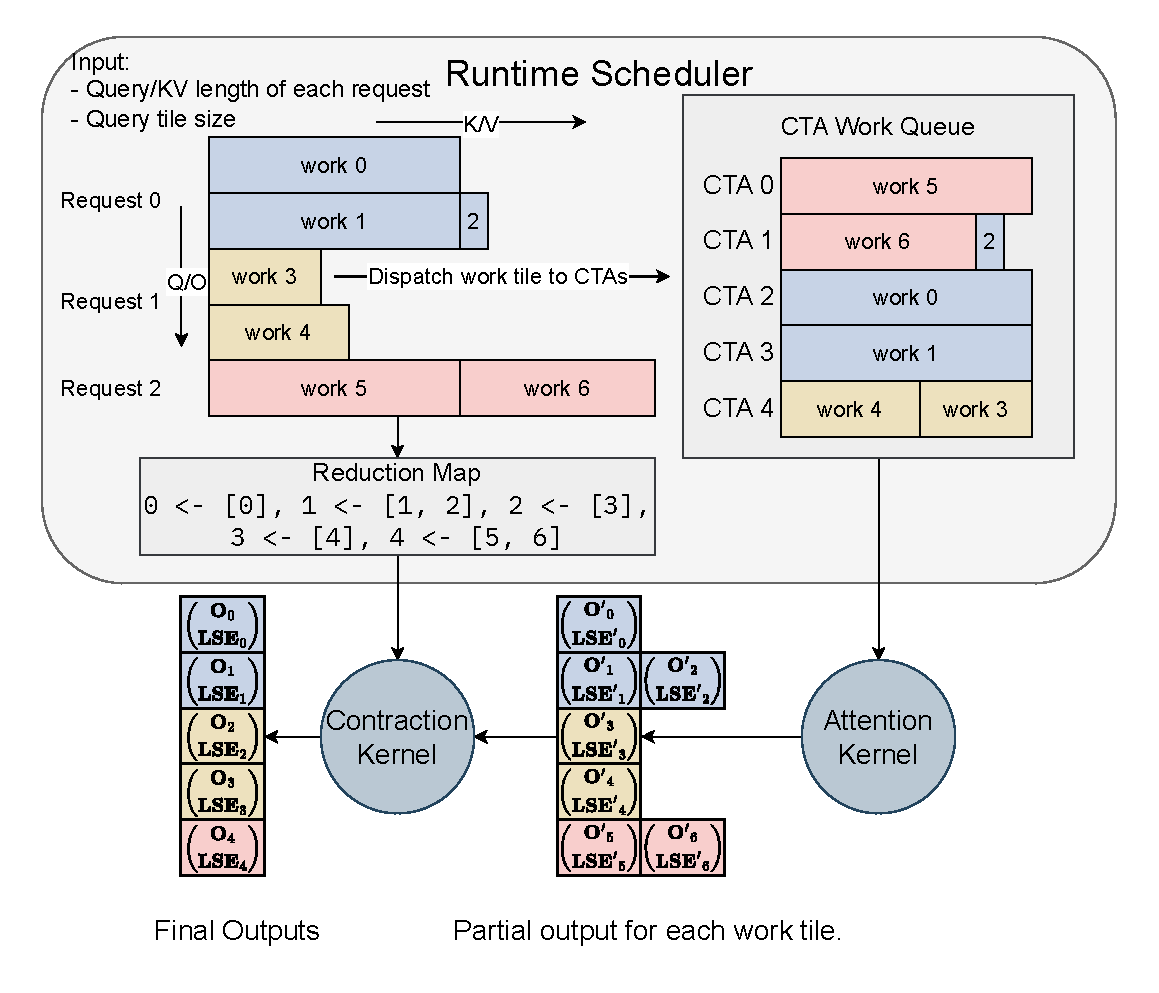
\includegraphics[width=0.4\textwidth]{figures/focus-scheduler.pdf}
    \caption{\sys 的负载均衡运行时调度器。query/output 与 key/value 两个维度的序列长度输入调度器后，生成计划信息：(1) 每个 CTA 的工作队列；(2) 部分输出与最终输出的索引映射。这些计划信息缓存于 GPU 侧，并作为持久化 attention/contraction 内核输入。}
    \centering
    \label{fig:flashinfer-scheduler}
\end{figure}

\sys 保证注意力阶段与收缩阶段均兼容 CUDAGraph~\cite{alan2019cudagraph,vinh2021pytorchcudagraph}。两个阶段都使用持久化内核，且 grid size 在编译后固定，即每个生成步都以相同 grid 启动。我们为 workspace buffer 的每个 section 设定固定偏移，用于存放部分输出与计划信息，确保每个生成步传入内核的指针保持一致，满足 CUDAGraph 要求（详见附录 \ref{sec:cudagraph-compatible-layout}）。我们还将两个阶段合并为一个持久化内核，消除内核间额外开销。

\subsection{编程接口}
\label{sec:programming-interface}

\sys 提供了面向集成的编程接口，可无缝接入 vLLM\cite{kwon2023vllm}、MLC-Engine\cite{mlcllm}、SGLang~\cite{zheng2023sglang} 等现有 LLM 服务框架。

\lstinputlisting[style=zihao-style, morekeywords={with}, label={lst:programming-interface}, caption={\sys 的 PyTorch 编程接口}]{code/programming_interface.py}

代码清单 \ref{lst:programming-interface} 展示了 \sys 的 PyTorch 接口。用户在初始化 wrapper 时提供注意力变体规格、任务信息和用户分配的 workspace buffer（详见附录 \ref{sec:memory-mgmt}），用于存储 \sys 动态调度所需的部分输出与计划信息。
内核在初始化时 JIT 编译并缓存复用。对于可组合格式（第 \ref{sec:composable-formats} 节），\sys 会创建多个注意力 wrapper，每个 wrapper 使用不同块大小。不同平均 query 长度与可组合格式配置对应的内核会分别编译，并捕获到不同 CUDAGraph 中。运行时，服务框架根据当前 KV-Cache 配置选择最合适的 CUDAGraph，从而在不同工作负载下保持最优性能。

\texttt{plan} 函数通过处理序列长度信息生成负载均衡调度计划，从而激活动态调度器。计划可缓存并在序列长度规格一致的算子间复用，例如同一生成步中的所有 decode attention。\texttt{run} 函数使用 query、key、value 与缓存计划执行注意力计算并输出结果。
CUDAGraph 可以捕获 \texttt{run} 调用并将整个注意力生成步骤编译为单图；但 \texttt{plan} 位于 CPU 侧，因此不会被 CUDAGraph 捕获。\texttt{plan}/\texttt{run} 的拆分受 Inspector-Executor（IE）模型~\cite{ravi1988principles, saltz1991preprocessed, ravi1993runtime} 启发，该模型被广泛用于并行化不规则工作负载。
